% =============================================================================
% Lecture 11: Feature Engineering for Business Forecasting
% BSAD 8310: Business Forecasting | University of Nebraska at Omaha
% =============================================================================
\documentclass[aspectratio=169, 10pt]{beamer}
% =============================================================================
% header.tex — BSAD 8310: Business Forecasting
% University of Nebraska at Omaha
% Beamer theme: UNO-branded, clean, professional
% =============================================================================

% ----------------------------- BEAMER THEME ----------------------------------
\usetheme{default}
\useinnertheme{rectangles}

% ----------------------------- UNO COLOR PALETTE -----------------------------
\definecolor{unoblue}{HTML}{005CA9}
\definecolor{unored}{HTML}{E41C38}
\definecolor{unogray}{HTML}{525252}
\definecolor{unogreen}{HTML}{15803d}
\definecolor{unolightblue}{HTML}{E8F0FA}
\definecolor{unolightred}{HTML}{FDECEA}
\definecolor{unolightgreen}{HTML}{F0FAF4}
\definecolor{unowhite}{HTML}{FFFFFF}

% Apply UNO colors to Beamer structure
\setbeamercolor{structure}{fg=unoblue}
\setbeamercolor{palette primary}{bg=unoblue, fg=white}
\setbeamercolor{palette secondary}{bg=unoblue!80!black, fg=white}
\setbeamercolor{palette tertiary}{bg=unoblue!60!black, fg=white}
\setbeamercolor{frametitle}{bg=unoblue, fg=white}
\setbeamercolor{frametitle right}{bg=unoblue!80!black}
\setbeamercolor{title}{fg=unoblue}
\setbeamercolor{subtitle}{fg=unogray}
\setbeamercolor{author in head/foot}{bg=unoblue, fg=white}
\setbeamercolor{title in head/foot}{bg=unoblue!80, fg=white}
\setbeamercolor{date in head/foot}{bg=unoblue!60, fg=white}
\setbeamercolor{page number in head/foot}{bg=unoblue!60, fg=white}
\setbeamercolor{block title}{bg=unoblue, fg=white}
\setbeamercolor{block body}{bg=unolightblue}
\setbeamercolor{block title alerted}{bg=unored, fg=white}
\setbeamercolor{block body alerted}{bg=unolightred}
\setbeamercolor{block title example}{bg=unogreen, fg=white}
\setbeamercolor{block body example}{bg=unolightgreen}
\setbeamercolor{itemize item}{fg=unoblue}
\setbeamercolor{itemize subitem}{fg=unored}
\setbeamercolor{enumerate item}{fg=unoblue}
\setbeamercolor{enumerate subitem}{fg=unored}
\setbeamercolor{alerted text}{fg=unored}

% ----------------------------- FONTS -----------------------------------------
\usefonttheme{professionalfonts}
\usefonttheme[onlymath]{serif}       % serif math; sans-serif text
\setbeamerfont{frametitle}{size=\large, series=\bfseries}
\setbeamerfont{title}{size=\LARGE, series=\bfseries}
\setbeamerfont{subtitle}{size=\large}
\setbeamerfont{block title}{size=\normalsize, series=\bfseries}
\setbeamerfont{footline}{size=\tiny}

% ----------------------------- LAYOUT ----------------------------------------
\setbeamersize{text margin left=0.5cm, text margin right=0.5cm}
\setbeamertemplate{navigation symbols}{}   % remove navigation buttons
\setbeamertemplate{itemize items}[circle]
\setbeamertemplate{enumerate items}[default]

% Custom footline: [Course] [Title] [Page/Total]
\setbeamertemplate{footline}{%
  \leavevmode%
  \hbox{%
    \begin{beamercolorbox}[wd=.33\paperwidth, ht=2.5ex, dp=1ex, left, leftskip=4pt]
      {author in head/foot}%
      \usebeamerfont{author in head/foot}\insertshortauthor
    \end{beamercolorbox}%
    \begin{beamercolorbox}[wd=.34\paperwidth, ht=2.5ex, dp=1ex, center]
      {title in head/foot}%
      \usebeamerfont{title in head/foot}\insertshorttitle
    \end{beamercolorbox}%
    \begin{beamercolorbox}[wd=.33\paperwidth, ht=2.5ex, dp=1ex, right, rightskip=4pt]
      {date in head/foot}%
      \usebeamerfont{date in head/foot}%
      \insertframenumber{} / \inserttotalframenumber
    \end{beamercolorbox}%
  }%
  \vskip0pt%
}

% Frametitle with thin accent line
\setbeamertemplate{frametitle}{%
  \vskip0.1cm
  \insertframetitle
  \vskip0.05cm
  \color{unored}\rule{\textwidth}{0.5pt}
}

% Title page
\setbeamertemplate{title page}{%
  \vfill
  \begin{center}
    {\color{unoblue}\rule{\textwidth}{2pt}}\\[0.3cm]
    {\usebeamerfont{title}\usebeamercolor[fg]{title}\inserttitle}\\[0.2cm]
    {\usebeamerfont{subtitle}\usebeamercolor[fg]{subtitle}\insertsubtitle}\\[0.3cm]
    {\color{unored}\rule{\textwidth}{0.5pt}}\\[0.4cm]
    {\small\insertauthor}\\[0.1cm]
    {\small\insertinstitute}\\[0.1cm]
    {\small\insertdate}
  \end{center}
  \vfill
}

% ----------------------------- PACKAGES --------------------------------------

% Math
\usepackage{amsmath}
\usepackage{amssymb}
\usepackage{mathtools}
\usepackage{bm}                    % bold math symbols

% Graphics & color
\usepackage{graphicx}
\usepackage{xcolor}
\usepackage{tikz}
\usetikzlibrary{arrows.meta, positioning, shapes, fit, backgrounds, calc}
\usepackage{pgfplots}
\pgfplotsset{compat=1.18}

% Tables
\usepackage{booktabs}
\usepackage{array}
\usepackage{multirow}
\usepackage{tabularx}

% Typography
\usepackage{microtype}
\usepackage{url}
\usepackage{hyperref}
\hypersetup{colorlinks=true, linkcolor=unoblue, urlcolor=unoblue, citecolor=unogray}

% Code listings (no shell-escape required)
\usepackage{listings}
\lstset{
  language=Python,
  basicstyle=\ttfamily\footnotesize,
  keywordstyle=\color{unoblue}\bfseries,
  stringstyle=\color{unogreen},
  commentstyle=\color{unogray}\itshape,
  numberstyle=\tiny\color{unogray},
  breaklines=true,
  showstringspaces=false,
  frame=single,
  rulecolor=\color{unogray!40},
  backgroundcolor=\color{unogray!5},
  xleftmargin=0.5em,
  xrightmargin=0.5em,
}

% Bibliography
\usepackage[backend=bibtex, style=authoryear, maxcitenames=2]{biblatex}
\addbibresource{../Bibliography_base.bib}

% Colored text helpers
\usepackage{tcolorbox}
\tcbuselibrary{skins, breakable, listingsutf8}

% ----------------------------- CUSTOM ENVIRONMENTS ---------------------------

% keybox: UNO-blue background — for key results, formulas, takeaways
\newtcolorbox{keybox}{
  enhanced,
  colback=unoblue,
  colframe=unoblue!80!black,
  coltitle=white,
  coltext=white,
  fonttitle=\bfseries,
  boxrule=0pt,
  arc=3pt,
  left=4pt, right=4pt, top=3pt, bottom=3pt,
}

% definitionbox: blue left-rule with title — for formal definitions
\newtcolorbox{definitionbox}[1]{
  enhanced,
  title={#1},
  colback=unolightblue,
  colframe=unoblue,
  coltitle=unoblue,
  fonttitle=\bfseries,
  boxrule=0pt,
  leftrule=3pt,
  arc=0pt,
  left=4pt, right=4pt, top=3pt, bottom=3pt,
}

% warningbox: red-accent — for pitfalls, assumption violations, common errors
\newtcolorbox{warningbox}{
  enhanced,
  colback=unolightred,
  colframe=unored,
  coltitle=white,
  fonttitle=\bfseries,
  boxrule=0pt,
  leftrule=3pt,
  arc=0pt,
  left=4pt, right=4pt, top=3pt, bottom=3pt,
}

% examplebox: green-accent with title — for worked examples, business applications
\newtcolorbox{examplebox}[1]{
  enhanced,
  title={#1},
  colback=unolightgreen,
  colframe=unogreen,
  coltitle=unogreen,
  fonttitle=\bfseries,
  boxrule=0pt,
  leftrule=3pt,
  arc=0pt,
  left=4pt, right=4pt, top=3pt, bottom=3pt,
}

% ----------------------------- MATH SHORTCUTS --------------------------------
\newcommand{\E}{\mathbb{E}}
\newcommand{\Var}{\operatorname{Var}}
\newcommand{\Cov}{\operatorname{Cov}}
\newcommand{\Corr}{\operatorname{Corr}}
\newcommand{\MSE}{\operatorname{MSE}}
\newcommand{\RMSE}{\operatorname{RMSE}}
\newcommand{\MAE}{\operatorname{MAE}}
\newcommand{\MASE}{\operatorname{MASE}}
\newcommand{\yhat}{\hat{y}}
\newcommand{\bhat}{\hat{\beta}}
\newcommand{\eps}{\varepsilon}
\newcommand{\given}{\,|\,}

% ----------------------------- SLIDE HELPERS ---------------------------------
% Section title slide (call at start of each section)
\newcommand{\sectionslide}[2]{%
  \begin{frame}
    \vfill
    \begin{center}
      {\color{unoblue}\rule{0.6\textwidth}{2pt}}\\[0.4cm]
      {\Large\bfseries\color{unoblue} #1}\\[0.2cm]
      {\normalsize\color{unogray} #2}\\[0.4cm]
      {\color{unored}\rule{0.6\textwidth}{1pt}}
    \end{center}
    \vfill
  \end{frame}
}

% Muted text
\newcommand{\muted}[1]{{\color{unogray}#1}}

% Key term
\newcommand{\key}[1]{{\color{unoblue}\textbf{#1}}}

% Positive / negative annotations
\newcommand{\pos}[1]{{\color{unogreen}#1}}
\newcommand{\negc}[1]{{\color{unored}#1}}


\title{Lecture 11: Feature Engineering}
\subtitle{Building Better Inputs for Forecasting Models}
\author{BSAD 8310: Business Forecasting}
\institute{University of Nebraska at Omaha}
\date{Spring 2026}

% =============================================================================
\begin{document}
% =============================================================================

\begin{frame}
  \titlepage
\end{frame}

\begin{frame}{Lecture Outline}
  \tableofcontents
\end{frame}

% -----------------------------------------------------------------------------
\begin{frame}{Motivation: The Feature Gap}
% -----------------------------------------------------------------------------
  \begin{keybox}
    \textbf{Lecture 10 best result:}
    LSTM with 36 features achieved RMSE $\approx$ 1,920 ---
    down from XGBoost's 2,250 (26 features).
    The improvement came mostly from \emph{better inputs}, not a
    fancier model.
  \end{keybox}

  \medskip
  \textbf{What feature engineering adds:}
  \begin{itemize}
    \item \textbf{Lag features:} give the model explicit access to
          past values, guided by ACF and PACF
    \item \textbf{Rolling statistics:} capture local trends,
          volatility, and momentum across multiple time scales
    \item \textbf{Calendar effects:} encode seasonality without
          requiring seasonal differencing
    \item \textbf{Interaction / ratio features:} year-over-year
          and month-over-month change rates that tree models cannot
          discover on their own
    \item \textbf{Pipeline design:} prevent data leakage by fitting
          transformations inside each cross-validation fold
  \end{itemize}

  \medskip
  \textbf{Lecture goal:} Build \texttt{make\_features\_extended()}
  (36 features), select the best subset, and update the
  Lectures 01--11 leaderboard.
\end{frame}

% =============================================================================
\section{Lag Features}
% =============================================================================

\sectionslide{Lag Features}{Converting time-series forecasting into a supervised regression problem}

\begin{frame}{Section Overview}
  \textbf{Lag features} are the most direct way to give a
  tree-based or linear model access to the past. They convert a
  time-series forecasting problem into a standard supervised
  regression problem with $y_{t-k}$ as predictors.

  \medskip
  \textbf{Design questions:}
  \begin{itemize}
    \item Which lags are worth including? (ACF and PACF guidance)
    \item How many lags before diminishing returns?
    \item How to avoid look-ahead leakage when computing lags?
  \end{itemize}

  \medskip
  \textbf{Key rule:} always use \texttt{shift(k)} with $k \geq 1$
  so that at prediction time for period $t$, only values observed at
  $t-1, t-2, \ldots$ are used.
\end{frame}

% -----------------------------------------------------------------------------
\begin{frame}{Choosing Lags: ACF and PACF Guidance}
% -----------------------------------------------------------------------------
  \begin{columns}[T]
    \begin{column}{0.52\textwidth}
      % ACF/PACF bar chart — hardcoded coords, no \foreach
      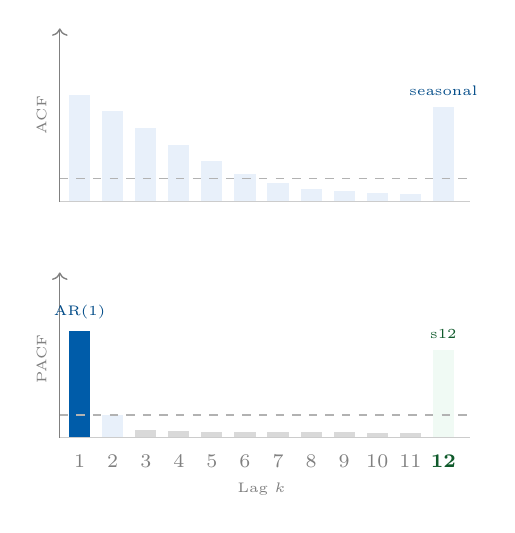
\begin{tikzpicture}[xscale=0.42, yscale=1.0]
        % ---- ACF panel (baseline y=3.0, max height 2.0) ----
        \fill[unolightblue] ( 0.68,3.0) rectangle ( 1.32,4.36);
        \fill[unolightblue] ( 1.68,3.0) rectangle ( 2.32,4.15);
        \fill[unolightblue] ( 2.68,3.0) rectangle ( 3.32,3.93);
        \fill[unolightblue] ( 3.68,3.0) rectangle ( 4.32,3.72);
        \fill[unolightblue] ( 4.68,3.0) rectangle ( 5.32,3.51);
        \fill[unolightblue] ( 5.68,3.0) rectangle ( 6.32,3.35);
        \fill[unolightblue] ( 6.68,3.0) rectangle ( 7.32,3.24);
        \fill[unolightblue] ( 7.68,3.0) rectangle ( 8.32,3.16);
        \fill[unolightblue] ( 8.68,3.0) rectangle ( 9.32,3.13);
        \fill[unolightblue] ( 9.68,3.0) rectangle (10.32,3.11);
        \fill[unolightblue] (10.68,3.0) rectangle (11.32,3.10);
        \fill[unolightblue] (11.68,3.0) rectangle (12.32,4.20);
        % ACF confidence band
        \draw[dashed, gray!60, line width=0.5pt]
              (0.4, 3.29) -- (12.8, 3.29);
        % ACF axis
        \draw[->, gray, line width=0.5pt]
              (0.4, 3.0) -- (0.4, 5.2);
        \node[font=\tiny, rotate=90, gray]
              at (-0.15, 4.1) {ACF};
        % ACF panel baseline
        \draw[gray!40, line width=0.4pt] (0.4,3.0) -- (12.8,3.0);
        % Lag 12 annotation
        \node[font=\tiny, text=unoblue!80!black, above]
              at (12.0, 4.22) {seasonal};

        % ---- PACF panel (baseline y=0.0, max height 2.0) ----
        \fill[unoblue]       ( 0.68,0.0) rectangle ( 1.32,1.36);
        \fill[unolightblue]  ( 1.68,0.0) rectangle ( 2.32,0.29);
        \fill[gray!30]       ( 2.68,0.0) rectangle ( 3.32,0.10);
        \fill[gray!30]       ( 3.68,0.0) rectangle ( 4.32,0.09);
        \fill[gray!30]       ( 4.68,0.0) rectangle ( 5.32,0.08);
        \fill[gray!30]       ( 5.68,0.0) rectangle ( 6.32,0.08);
        \fill[gray!30]       ( 6.68,0.0) rectangle ( 7.32,0.07);
        \fill[gray!30]       ( 7.68,0.0) rectangle ( 8.32,0.07);
        \fill[gray!30]       ( 8.68,0.0) rectangle ( 9.32,0.07);
        \fill[gray!30]       ( 9.68,0.0) rectangle (10.32,0.06);
        \fill[gray!30]       (10.68,0.0) rectangle (11.32,0.06);
        \fill[unolightgreen] (11.68,0.0) rectangle (12.32,1.12);
        % PACF confidence band
        \draw[dashed, gray!60, line width=0.5pt]
              (0.4, 0.29) -- (12.8, 0.29);
        % PACF axis
        \draw[->, gray, line width=0.5pt]
              (0.4, 0.0) -- (0.4, 2.1);
        \node[font=\tiny, rotate=90, gray]
              at (-0.15, 1.0) {PACF};
        % PACF panel baseline
        \draw[gray!40, line width=0.4pt] (0.4,0.0) -- (12.8,0.0);
        % Lag 1 PACF annotation
        \node[font=\tiny, text=unoblue!80!black, above]
              at (1.0, 1.38) {AR(1)};
        % Lag 12 PACF annotation
        \node[font=\tiny, text=unogreen!70!black, above]
              at (12.0, 1.14) {s12};
        % x-axis labels
        \node[font=\scriptsize, gray] at ( 1.0,-0.30) {1};
        \node[font=\scriptsize, gray] at ( 2.0,-0.30) {2};
        \node[font=\scriptsize, gray] at ( 3.0,-0.30) {3};
        \node[font=\scriptsize, gray] at ( 4.0,-0.30) {4};
        \node[font=\scriptsize, gray] at ( 5.0,-0.30) {5};
        \node[font=\scriptsize, gray] at ( 6.0,-0.30) {6};
        \node[font=\scriptsize, gray] at ( 7.0,-0.30) {7};
        \node[font=\scriptsize, gray] at ( 8.0,-0.30) {8};
        \node[font=\scriptsize, gray] at ( 9.0,-0.30) {9};
        \node[font=\scriptsize, gray] at (10.0,-0.30) {10};
        \node[font=\scriptsize, gray] at (11.0,-0.30) {11};
        \node[font=\scriptsize, text=unogreen!70!black]
              at (12.0,-0.30) {\textbf{12}};
        \node[font=\tiny, gray] at (6.5,-0.65) {Lag $k$};
      \end{tikzpicture}
    \end{column}
    \begin{column}{0.44\textwidth}
      \textbf{Reading the charts:}
      \begin{itemize}
        \item \textbf{ACF:} slow decay → persistent trend;
              spike at lag 12 → seasonal pattern
        \item \textbf{PACF:} significant at lag 1 only →
              pure AR(1); significant at lag 12 →
              include \texttt{lag\_12}
      \end{itemize}

      \begin{definitionbox}{Lag Selection Rule}
        \footnotesize
        Include \texttt{lag\_k} if the PACF at lag $k$
        exceeds $\pm 1.96/\sqrt{n}$ (dashed band).
        For monthly RSXFS: include lags 1, 2, 12.
        Add lags 3--6 for robustness.
      \end{definitionbox}

      \smallskip
      \muted{\footnotesize\itshape
        Socratic: ACF at lag 12 is strong, but PACF at
        lag 12 is also strong. Why include \texttt{lag\_12}
        even in an ARIMA model that handles seasonality
        through differencing?}
    \end{column}
  \end{columns}
\end{frame}

% -----------------------------------------------------------------------------
\begin{frame}[fragile]{Lag Leakage: Safe Shift vs.\ Lookahead Bug}
% -----------------------------------------------------------------------------
  \begin{columns}[T]
    \begin{column}{0.48\textwidth}
      \textbf{Safe: always \texttt{shift(k)}}
\begin{lstlisting}[language=Python,
                   basicstyle=\tiny\ttfamily]
import pandas as pd

# SAFE: shift(k) looks back k steps
# At time t we only see y[t-k]
df['lag_1']  = df['y'].shift(1)
df['lag_2']  = df['y'].shift(2)
df['lag_12'] = df['y'].shift(12)

# Rolling mean: shift FIRST
df['roll_mean_3'] = (
    df['y'].shift(1)
    .rolling(3).mean())

# No future information used.
print("Lag features are safe.")
\end{lstlisting}
    \end{column}
    \begin{column}{0.48\textwidth}
      \textbf{Bug: missing \texttt{shift(1)}}
\begin{lstlisting}[language=Python,
                   basicstyle=\tiny\ttfamily]
# BUG: rolling without shift(1)
# includes y[t] = current target!
df['roll_mean_3'] = (
    df['y'].rolling(3).mean())

# At t=5, rolling uses:
#   y[3], y[4], y[5]  <- leakage!
# y[5] is what we are predicting.

# This inflates in-sample R^2
# but collapses on test data.

# Rule: always shift before
# any window operation.
\end{lstlisting}
      \smallskip
      \begin{warningbox}
        \footnotesize
        Rolling without \texttt{shift(1)} is the
        \#1 feature engineering bug. It causes
        dramatic overfitting that only appears on
        the test set.
      \end{warningbox}
    \end{column}
  \end{columns}
\end{frame}

% =============================================================================
\section{Rolling Statistics}
% =============================================================================

\sectionslide{Rolling Statistics}{Local trends, volatility, and momentum over time}

\begin{frame}{Section Overview}
  \textbf{Rolling statistics} capture local trends, volatility,
  and momentum over multiple time windows. They are especially
  powerful for tree-based models, which cannot express the concept
  of a ``moving average'' from raw lag features alone.

  \medskip
  \textbf{Feature families:}
  \begin{itemize}
    \item \textbf{Rolling mean} ($w = 3, 6, 12$): local trend
          at multiple scales
    \item \textbf{Rolling std} ($w = 3, 6, 12$): local
          volatility --- useful for identifying calm vs.\ volatile
          regimes
    \item \textbf{Rolling min/max} ($w = 3, 6, 12$): range and
          extremes
    \item \textbf{Exponentially weighted mean (EWM)}: gives
          more weight to recent observations than a simple average
  \end{itemize}

  \medskip
  All rolling operations must be computed on
  \texttt{df['value'].shift(1)} to prevent leakage
  (see the Lag Leakage slide).
\end{frame}

% -----------------------------------------------------------------------------
\begin{frame}{Rolling Statistics and EWM}
% -----------------------------------------------------------------------------
  \begin{columns}[T]
    \begin{column}{0.52\textwidth}
      \textbf{Rolling window operations:}
      \begin{center}
      \footnotesize
      \begin{tabular}{lll}
        \toprule
        \textbf{Feature} & \textbf{Formula} & \textbf{Captures} \\
        \midrule
        \texttt{roll\_mean\_w} & $\bar{y}_{t-w:t-1}$
                               & Local trend \\
        \texttt{roll\_std\_w}  & $s_{t-w:t-1}$
                               & Volatility \\
        \texttt{roll\_min\_w}  & $\min(y_{t-w},\ldots,y_{t-1})$
                               & Trough \\
        \texttt{roll\_max\_w}  & $\max(y_{t-w},\ldots,y_{t-1})$
                               & Peak \\
        \bottomrule
      \end{tabular}
      \end{center}

      \medskip
      \textbf{Exponentially weighted mean:}
      \[
        \mathrm{EWM}_t
          = \alpha\, y_{t-1}
          + (1-\alpha)\,\mathrm{EWM}_{t-1},
          \quad \alpha \in (0,1)
      \]
      With $\alpha = 0.3$: recent values receive
      ${\approx}3\times$ the weight of values 4 months back.

      \smallskip
      \muted{\footnotesize\itshape
        Here $\alpha$ is the EWM decay weight ---
        distinct from the level-smoothing $\alpha$ in Lecture~03
        (ETS) and the L1/L2 mixing $\alpha$ in Lecture~08
        (Elastic Net).}
    \end{column}
    \begin{column}{0.44\textwidth}
      \begin{definitionbox}{Window Choice Heuristics}
        \footnotesize
        \begin{itemize}
          \item $w = 3$: captures quarter-long momentum
          \item $w = 6$: captures half-year cycles
          \item $w = 12$: captures full-year seasonality
        \end{itemize}
        Use all three; let the model select via
        regularization or feature importance.
      \end{definitionbox}

      \smallskip
      \begin{examplebox}{EWM vs.\ Rolling Mean}
        \footnotesize
        EWM reacts faster to trend reversals.
        On RSXFS, EWM with $\alpha=0.3$ reduces
        lag behind turning points by $\sim$2 months
        compared with a 12-month rolling mean.
      \end{examplebox}
    \end{column}
  \end{columns}
\end{frame}

% -----------------------------------------------------------------------------
\begin{frame}{Which Features Matter? A Preview}
% -----------------------------------------------------------------------------
  \begin{columns}[T]
    \begin{column}{0.54\textwidth}
      % Permutation importance bar chart — hardcoded, no \foreach
      \textbf{Permutation importance (Random Forest, val set):}

      \smallskip
      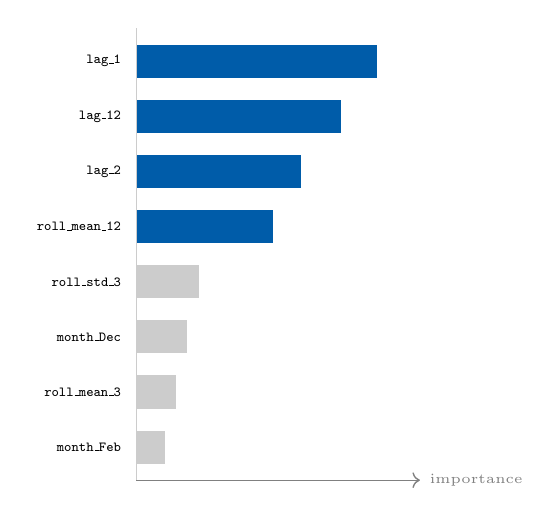
\begin{tikzpicture}[xscale=3.6, yscale=0.70]
        % Top 4 features (unoblue)
        \fill[unoblue] (0, 7.7) rectangle (0.85, 8.3);
        \fill[unoblue] (0, 6.7) rectangle (0.72, 7.3);
        \fill[unoblue] (0, 5.7) rectangle (0.58, 6.3);
        \fill[unoblue] (0, 4.7) rectangle (0.48, 5.3);
        % Bottom 4 features (gray!40)
        \fill[gray!40] (0, 3.7) rectangle (0.22, 4.3);
        \fill[gray!40] (0, 2.7) rectangle (0.18, 3.3);
        \fill[gray!40] (0, 1.7) rectangle (0.14, 2.3);
        \fill[gray!40] (0, 0.7) rectangle (0.10, 1.3);
        % Feature labels
        \node[font=\tiny, anchor=east]
          at (-0.02, 8.0) {\texttt{lag\_1}};
        \node[font=\tiny, anchor=east]
          at (-0.02, 7.0) {\texttt{lag\_12}};
        \node[font=\tiny, anchor=east]
          at (-0.02, 6.0) {\texttt{lag\_2}};
        \node[font=\tiny, anchor=east]
          at (-0.02, 5.0) {\texttt{roll\_mean\_12}};
        \node[font=\tiny, anchor=east]
          at (-0.02, 4.0) {\texttt{roll\_std\_3}};
        \node[font=\tiny, anchor=east]
          at (-0.02, 3.0) {\texttt{month\_Dec}};
        \node[font=\tiny, anchor=east]
          at (-0.02, 2.0) {\texttt{roll\_mean\_3}};
        \node[font=\tiny, anchor=east]
          at (-0.02, 1.0) {\texttt{month\_Feb}};
        % x-axis
        \draw[->, gray, line width=0.5pt]
          (0, 0.4) -- (1.0, 0.4)
          node[right, font=\tiny, gray]
          {importance};
        % Vertical line at x=0
        \draw[gray!40, line width=0.4pt]
          (0, 0.4) -- (0, 8.6);
      \end{tikzpicture}
    \end{column}
    \begin{column}{0.42\textwidth}
      \textbf{Key findings:}
      \begin{itemize}
        \item Lags 1 and 12 dominate --- confirming ACF/PACF
        \item \texttt{roll\_mean\_12} is the most important
              rolling feature
        \item \texttt{month\_Dec} matters: December retail
              spike is real
        \item Calendar dummies are less important than
              rolling features when lags already capture
              seasonal levels
      \end{itemize}

      \medskip
      \muted{\footnotesize\itshape
        This ranking is illustrative. Permutation
        importance is covered formally in Section 5
        (Feature Selection).}
    \end{column}
  \end{columns}
\end{frame}

% =============================================================================
\section{Calendar and Structural Features}
% =============================================================================

\sectionslide{Calendar \& Structural Features}{Encoding temporal position for tree-based models}

\begin{frame}{Section Overview}
  \textbf{Calendar features} encode the position of a time step
  in the calendar --- month, quarter, year, holiday proximity.
  Unlike SARIMA's seasonal differencing, calendar dummies give
  tree-based models explicit information about which periods are
  structurally different.

  \medskip
  \textbf{Key feature types:}
  \begin{itemize}
    \item \textbf{Month dummies:} 11 binary columns
          (\texttt{month\_2} through \texttt{month\_12});
          January is the reference category
    \item \textbf{Quarter dummies:} 3 binary columns (Q2--Q4)
    \item \textbf{Trend term:} $t = 1, 2, \ldots, T$
          for linear time trend
    \item \textbf{Structural break indicator:} 0/1 for
          pre/post a known break (recession, pandemic, policy
          change)
  \end{itemize}
\end{frame}

% -----------------------------------------------------------------------------
\begin{frame}{Month Dummies: Construction and Interpretation}
% -----------------------------------------------------------------------------
  \begin{columns}[T]
    \begin{column}{0.52\textwidth}
      \textbf{Construction in pandas:}

      \smallskip
      \footnotesize
      \texttt{df.index.month} $\rightarrow$ integers 1--12 \\[4pt]
      \texttt{pd.get\_dummies(df['month'], prefix='month',
      drop\_first=True)}

      \bigskip
      \textbf{Interpretation (Random Forest):}
      \begin{center}
      \footnotesize
      \begin{tabular}{lrr}
        \toprule
        \textbf{Month} & \textbf{Avg.\ Effect}
                       & \textbf{Business Meaning} \\
        \midrule
        January (ref) & ---    & Post-holiday low \\
        \texttt{month\_11}     & $+$1,800 & Nov.\ ramp-up \\
        \texttt{month\_12}     & $+$3,200 & Holiday peak \\
        \texttt{month\_7}      & $+$900   & Summer surge \\
        \texttt{month\_2}      & $-$400   & Feb.\ dip \\
        \bottomrule
      \end{tabular}
      \end{center}
    \end{column}
    \begin{column}{0.44\textwidth}
      \begin{examplebox}{Calendar vs.\ Seasonal Lag}
        \footnotesize
        \textbf{Both encode seasonality, but differently:}
        \begin{itemize}
          \item \texttt{lag\_12} $= y_{t-12}$: level effect ---
                captures the same magnitude as last year
          \item \texttt{month\_12}: indicator effect ---
                always adds the same fixed amount for
                December, regardless of last year's level
        \end{itemize}
        Use both when trend is changing.
      \end{examplebox}

      \smallskip
      \muted{\footnotesize\itshape
        Socratic: A SARIMA model with $s=12$ handles
        seasonality through seasonal differencing.
        Why might month dummies improve a Random Forest
        but add no value to SARIMA?}
    \end{column}
  \end{columns}
\end{frame}

% -----------------------------------------------------------------------------
\begin{frame}{When Calendar Features Help and Hurt}
% -----------------------------------------------------------------------------
  \begin{columns}[T]
    \begin{column}{0.48\textwidth}
      \textbf{Calendar features help when:}
      \begin{itemize}
        \item The seasonal pattern is \emph{fixed} across years
              (e.g., holiday retail, fiscal quarters)
        \item The model does not already capture seasonality
              via lag features (e.g., shallow trees, linear
              models without lag 12)
        \item Structural breaks are known and datable
              (add a 0/1 indicator for pre/post)
      \end{itemize}
    \end{column}
    \begin{column}{0.48\textwidth}
      \textbf{Calendar features can hurt when:}
      \begin{itemize}
        \item Seasonal patterns are \emph{evolving} over time
              --- the fixed-effect assumption breaks down
        \item \texttt{lag\_12} already accounts for
              seasonality --- month dummies add multicollinearity
        \item The dataset is small ($n < 100$): 11 month
              dummies consume degrees of freedom faster than
              they add signal
      \end{itemize}
    \end{column}
  \end{columns}

  \medskip
  \begin{warningbox}
    Never use calendar dummies as the sole source of seasonality
    in a neural network (LSTM). LSTMs learn temporal patterns from
    the sequence itself; adding 11 overlapping dummies adds noise.
    Use them as supplementary features only when lag features are
    already present.
  \end{warningbox}
\end{frame}

% =============================================================================
\section{Interaction and Ratio Features}
% =============================================================================

\sectionslide{Interaction \& Ratio Features}{Encoding change, not level}

\begin{frame}{Section Overview}
  \textbf{Interaction and ratio features} encode \emph{change}
  rather than \emph{level}. They help tree-based models detect
  acceleration or deceleration in a series --- a concept that
  requires computing ratios of two variables, something a single
  tree split cannot express directly.

  \medskip
  \textbf{Key features:}
  \begin{itemize}
    \item \textbf{Year-over-year (YoY) change:}
          $\Delta^{(12)} y_t = y_{t-1} / y_{t-13} - 1$
    \item \textbf{Month-over-month (MoM) change:}
          $\Delta^{(1)} y_t = y_{t-1} / y_{t-2} - 1$
    \item \textbf{Lag interaction:}
          $y_{t-1} \times \mathbf{1}[\text{month} = 12]$ ---
          lets the model use different slopes for December
  \end{itemize}
\end{frame}

% -----------------------------------------------------------------------------
\begin{frame}{Year-Over-Year and Month-Over-Month Formulas}
% -----------------------------------------------------------------------------
  \begin{columns}[T]
    \begin{column}{0.50\textwidth}
      \textbf{Year-over-year rate of change:}
      \[
        \text{YoY}_t
          = \frac{y_{t-1}}{y_{t-13}} - 1
      \]
      Note: both $y_{t-1}$ and $y_{t-13}$ are lagged to
      prevent leakage at prediction time for target $y_t$.

      \medskip
      \textbf{Month-over-month rate of change:}
      \[
        \text{MoM}_t
          = \frac{y_{t-1}}{y_{t-2}} - 1
      \]
      \textbf{Why ratios instead of differences?}
      A 1,000-unit change means something different when
      the baseline is 10,000 vs.\ 100,000.
      Ratios are scale-free.
    \end{column}
    \begin{column}{0.46\textwidth}
      \begin{definitionbox}{Economic Interpretation}
        \footnotesize
        For RSXFS retail sales:
        \begin{itemize}
          \item $\text{YoY}_t > 0$: economy is stronger
                than same month last year
          \item $\text{YoY}_t < 0$: contraction signal
          \item $|\text{MoM}_t|$ large: abnormal
                month-to-month swing (data revision or
                shock)
        \end{itemize}
        These features help the model distinguish a
        Christmas peak from an unexpected demand shock.
      \end{definitionbox}

      \medskip
      \muted{\footnotesize\itshape
        Socratic: YoY removes the seasonal level but
        still contains trend. What additional
        transformation would make $\text{YoY}_t$ a
        stationary series?}
    \end{column}
  \end{columns}
\end{frame}

% -----------------------------------------------------------------------------
\begin{frame}[fragile]{The Extended Feature Function (36 Features)}
% -----------------------------------------------------------------------------
  \textbf{Full feature engineering pipeline:}
  \smallskip
\begin{lstlisting}[language=Python, basicstyle=\tiny\ttfamily]
def make_features_extended(df,
                            lags=range(1, 13),
                            roll_windows=[3, 6, 12]):
    X = df[['value']].copy()
    # Lag features (ACF/PACF-guided, lags 1--12)
    for k in lags:
        X[f'lag_{k}'] = X['value'].shift(k)
    # Rolling stats (shift first to avoid leakage)
    for w in roll_windows:
        r = X['value'].shift(1).rolling(w)
        X[f'roll_mean_{w}'] = r.mean()
        X[f'roll_std_{w}']  = r.std()
        X[f'roll_min_{w}']  = r.min()
        X[f'roll_max_{w}']  = r.max()
    # Exponentially weighted mean
    X['ewm_alpha03'] = (
        X['value'].shift(1)
        .ewm(alpha=0.3, adjust=False).mean())
    # Calendar dummies (Jan = reference category)
    months = pd.Series(
        X.index.month, index=X.index)
    dums = pd.get_dummies(
        months, prefix='month',
        drop_first=True)
    X = pd.concat([X, dums], axis=1)
    # Return 36-column feature matrix
    return X.drop(columns='value').dropna()
\end{lstlisting}
\end{frame}

% =============================================================================
\section{Feature Selection}
% =============================================================================

\sectionslide{Feature Selection}{Choosing the best subset of 36 candidate features}

\begin{frame}{Section Overview}
  More features are not always better. With 36 features and
  $n \approx 300$ observations, we risk overfitting --- especially
  in linear models. \textbf{Feature selection} identifies the
  subset of features that maximizes out-of-sample predictive
  accuracy.

  \medskip
  \textbf{Three strategies covered today:}
  \begin{enumerate}
    \item \textbf{LASSO} (from Lecture 08): $\ell_1$ penalty
          shrinks irrelevant feature coefficients to exactly zero.
          Implicit selection via the regularization path.
    \item \textbf{Permutation importance}: measure how much
          test RMSE rises when a feature's values are randomly
          shuffled. Model-agnostic
    \item \textbf{RFECV}: Recursive Feature Elimination with
          cross-validation. Fit model, remove weakest feature,
          repeat until CV score stops improving
  \end{enumerate}
\end{frame}

% -----------------------------------------------------------------------------
\begin{frame}{Feature Selection via LASSO}
% -----------------------------------------------------------------------------
  \textbf{LASSO regularization path} (Lecture 08 connection):
  \[
    \hat{\boldsymbol{\beta}}^{\text{LASSO}}
      = \operatorname{arg\,min}_{\boldsymbol{\beta}}
        \underbrace{\sum_{t} (y_t - \mathbf{x}_t^\top \boldsymbol{\beta})^2}_{\text{prediction error}}
        + \lambda \underbrace{\|\boldsymbol{\beta}\|_1}_{\text{selection penalty}}
  \]

  \medskip
  As $\lambda$ increases along the regularization path:
  \begin{itemize}
    \item \textbf{Lag 12 and lag 1} coefficients survive to large $\lambda$ ---
          high marginal importance
    \item \textbf{Rolling std features} shrink toward zero early ---
          lower marginal importance
    \item At CV-optimal $\lambda^*$: many coefficients are exactly zero
          (automatic feature selection) \parencite{Tibshirani1996}
  \end{itemize}

  \medskip
  \muted{\footnotesize\itshape
    LASSO requires standardized features --- all inputs should be
    on comparable scales (use \texttt{StandardScaler} inside a
    \texttt{Pipeline} to prevent leakage).}
\end{frame}

% -----------------------------------------------------------------------------
\begin{frame}{Feature Selection via Permutation Importance}
% -----------------------------------------------------------------------------
  \begin{definitionbox}{Algorithm: Permutation Importance \parencite{Molnar2022}}
    \footnotesize
    \begin{enumerate}
      \item Fit Random Forest on training set
      \item Record \textbf{baseline} validation RMSE: $\text{RMSE}_0$
      \item For each feature $j$: shuffle column $j$, re-predict,
            record $\text{RMSE}_j$
      \item $\text{Importance}_j = \text{RMSE}_j - \text{RMSE}_0$
            \quad (larger = more important)
    \end{enumerate}
  \end{definitionbox}

  \medskip
  \textbf{Advantages over split-count (impurity) importance:}
  \begin{itemize}
    \item Evaluated on \emph{validation} set --- not biased toward
          high-cardinality features
    \item \emph{Model-agnostic}: applies to LSTM, XGBoost, linear models
    \item Measures \emph{marginal} contribution with all other features present
  \end{itemize}

  \medskip
  \muted{\footnotesize\itshape
    On RSXFS: \texttt{lag\_1}, \texttt{lag\_12}, \texttt{roll\_mean\_12},
    \texttt{ewm\_alpha03} are the top four. See the importance preview
    in Section 2 (Rolling Statistics).}
\end{frame}

% -----------------------------------------------------------------------------
\begin{frame}[fragile]{RFECV: Recursive Feature Elimination}
% -----------------------------------------------------------------------------
  \begin{columns}[T]
    \begin{column}{0.49\textwidth}
      \begin{definitionbox}{RFECV Algorithm}
        \footnotesize
        \textbf{Input:} estimator, feature matrix $X$,
        cross-validator\\[3pt]
        \textbf{Repeat:}
        \begin{enumerate}
          \item Fit estimator on all remaining features
          \item Rank features by importance
          \item Eliminate the lowest-ranked feature
        \end{enumerate}
        \textbf{Select:} the subset size that maximizes
        mean CV score \parencite{Guyon2003}
      \end{definitionbox}

      \textbf{Key parameters:}
      \begin{itemize}
        \item \texttt{step=1}: eliminate one feature
              per round
        \item \texttt{cv=TimeSeriesSplit(gap=1)}:
              prevents temporal leakage during selection
        \item \texttt{min\_features\_to\_select=5}:
              floor to avoid trivial models
      \end{itemize}
    \end{column}
    \begin{column}{0.48\textwidth}
\begin{lstlisting}[language=Python,
                   basicstyle=\tiny\ttfamily]
from sklearn.feature_selection import RFECV
from sklearn.ensemble import (
    RandomForestRegressor)
from sklearn.model_selection import (
    TimeSeriesSplit)

estimator = RandomForestRegressor(
    n_estimators=200, random_state=42)

tscv = TimeSeriesSplit(n_splits=5, gap=1)

selector = RFECV(
    estimator=estimator,
    step=1,
    cv=tscv,
    scoring='neg_mean_squared_error',
    min_features_to_select=5)

selector.fit(X_tr, y_tr)

# Selected feature names
selected = X_tr.columns[
    selector.support_].tolist()
print(f"Selected: {len(selected)} feats")
\end{lstlisting}
    \end{column}
  \end{columns}
\end{frame}

% =============================================================================
\section{Pipeline Design}
% =============================================================================

\sectionslide{Pipeline Design}{Preventing leakage in cross-validation}

\begin{frame}{Section Overview}
  A \textbf{sklearn Pipeline} chains transformations and a model
  into a single object. Inside cross-validation, the pipeline
  re-fits every transformation on the training fold only ---
  preventing the subtle leakage that occurs when scaling with
  statistics from the full dataset.

  \medskip
  \textbf{Why pipelines matter for time-series CV:}
  \begin{itemize}
    \item \texttt{StandardScaler} fitted on all data
          leaks test-set mean and variance into training
    \item With \texttt{Pipeline} + \texttt{TimeSeriesSplit}:
          scaler is fitted fresh on each train fold
    \item Same principle applies to \texttt{RFECV} and
          any imputer --- fit only on train, transform both
          train and test \parencite{Pedregosa2011}
  \end{itemize}

  \medskip
  \muted{\footnotesize\itshape
    Rule of thumb: if a transformation looks at the target
    variable (e.g., LabelEncoder, WoE encoding) or at the
    distribution of $X$ (e.g., StandardScaler, PCA), it
    \emph{must} go inside the pipeline.}
\end{frame}

% -----------------------------------------------------------------------------
\begin{frame}{Pipeline Flow: From Features to Predictions}
% -----------------------------------------------------------------------------
  \begin{columns}[T]
    \begin{column}{0.44\textwidth}
      % Pipeline flow diagram — 6 stages, hardcoded y-coords
      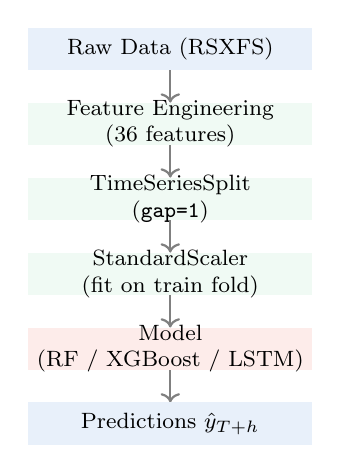
\begin{tikzpicture}[xscale=0.95, yscale=0.68]
        % Stage 1: Raw data (unolightblue)
        \fill[unolightblue]  (0, 9.6) rectangle (3.8, 10.4);
        \node[font=\footnotesize, align=center]
          at (1.9, 10.0) {Raw Data (RSXFS)};
        % Arrow 1→2
        \draw[->, gray, line width=0.8pt]
          (1.9, 9.6) -- (1.9, 9.0);
        % Stage 2: Feature engineering (unolightgreen)
        \fill[unolightgreen] (0, 8.2) rectangle (3.8, 9.0);
        \node[font=\footnotesize, align=center]
          at (1.9, 8.6) {Feature Engineering\\(36 features)};
        % Arrow 2→3
        \draw[->, gray, line width=0.8pt]
          (1.9, 8.2) -- (1.9, 7.6);
        % Stage 3: TimeSeriesSplit (unolightgreen)
        \fill[unolightgreen] (0, 6.8) rectangle (3.8, 7.6);
        \node[font=\footnotesize, align=center]
          at (1.9, 7.2) {TimeSeriesSplit\\(\texttt{gap=1})};
        % Arrow 3→4
        \draw[->, gray, line width=0.8pt]
          (1.9, 6.8) -- (1.9, 6.2);
        % Stage 4: StandardScaler (unolightgreen)
        \fill[unolightgreen] (0, 5.4) rectangle (3.8, 6.2);
        \node[font=\footnotesize, align=center]
          at (1.9, 5.8) {StandardScaler\\(fit on train fold)};
        % Arrow 4→5
        \draw[->, gray, line width=0.8pt]
          (1.9, 5.4) -- (1.9, 4.8);
        % Stage 5: Model (unolightred)
        \fill[unolightred]   (0, 4.0) rectangle (3.8, 4.8);
        \node[font=\footnotesize, align=center]
          at (1.9, 4.4) {Model\\(RF / XGBoost / LSTM)};
        % Arrow 5→6
        \draw[->, gray, line width=0.8pt]
          (1.9, 4.0) -- (1.9, 3.4);
        % Stage 6: Predictions (unolightblue)
        \fill[unolightblue]  (0, 2.6) rectangle (3.8, 3.4);
        \node[font=\footnotesize, align=center]
          at (1.9, 3.0) {Predictions $\hat{y}_{T+h}$};
      \end{tikzpicture}
    \end{column}
    \begin{column}{0.52\textwidth}
      \textbf{What happens inside each CV fold:}
      {\footnotesize\begin{enumerate}
        \item \textbf{Split:} \texttt{TimeSeriesSplit(gap=1)}
              --- 1-step gap prevents leakage
        \item \textbf{Fit scaler:} \texttt{StandardScaler}
              on train fold \emph{only}
        \item \textbf{Transform:} same params applied
              to train and val
        \item \textbf{Fit model:} on scaled train fold
        \item \textbf{Score:} RMSE on scaled val fold
        \item \textbf{Report:} average across all folds
      \end{enumerate}}

      \begin{examplebox}{The Leakage Trap}
        \footnotesize
        Fitting \texttt{StandardScaler} before CV
        on all data: validation mean/std seep into
        training. Typical RMSE improvement from
        fixing this: 50--200 units on RSXFS.
      \end{examplebox}
    \end{column}
  \end{columns}
\end{frame}

% -----------------------------------------------------------------------------
\begin{frame}[fragile]{Building a Leakage-Free Pipeline}
% -----------------------------------------------------------------------------
  \begin{columns}[T]
    \begin{column}{0.50\textwidth}
      \textbf{Step 1: Construct the pipeline}
\begin{lstlisting}[language=Python,
                   basicstyle=\tiny\ttfamily]
from sklearn.pipeline import Pipeline
from sklearn.preprocessing import (
    StandardScaler)
from sklearn.ensemble import (
    RandomForestRegressor)
from sklearn.model_selection import (
    TimeSeriesSplit, cross_val_score)
import numpy as np

# Build pipeline (order matters!)
pipe = Pipeline([
    ('scaler', StandardScaler()),
    ('model', RandomForestRegressor(
        n_estimators=300,
        random_state=42))])

tscv = TimeSeriesSplit(
    n_splits=5, gap=1)
\end{lstlisting}
    \end{column}
    \begin{column}{0.47\textwidth}
      \textbf{Step 2: Cross-validate and predict}
\begin{lstlisting}[language=Python,
                   basicstyle=\tiny\ttfamily]
# CV: scaler fit on each train fold
scores = cross_val_score(
    pipe,
    X.values,
    y.values,
    cv=tscv,
    scoring=(
        'neg_mean_squared_error'))
rmse_cv = np.sqrt(-scores.mean())
print(f"CV RMSE: {rmse_cv:,.0f}")

# Refit on full training data
pipe.fit(X_tr.values, y_tr.values)

# Predict on held-out test set
y_pred = pipe.predict(
    X_te.values)
rmse_te = np.sqrt(
    np.mean((y_te - y_pred)**2))
print(f"Test RMSE: {rmse_te:,.0f}")
\end{lstlisting}
    \end{column}
  \end{columns}
\end{frame}

% =============================================================================
\section{Application to Forecasting}
% =============================================================================

\sectionslide{Application to Forecasting}{Baseline vs.\ extended features on RSXFS retail sales}

\begin{frame}{Section Overview}
  Apply \texttt{make\_features\_extended()} (36 features) to
  RSXFS retail sales and compare against the baseline 26-feature
  set from Lectures 07--10. Measure the marginal contribution of
  better features holding the model class fixed.

  \medskip
  \textbf{Evaluation design:}
  \begin{itemize}
    \item \textbf{Baseline} (26 features): 12 lags, 6 rolling
          means, 6 rolling stds, 2 ratios --- as in Lectures 07--10
    \item \textbf{Extended} (36 features): adds rolling min/max,
          EWM, and 11 month dummies
    \item \textbf{Models:} Elastic Net, Random Forest, XGBoost,
          LSTM (median over 5 seeds)
    \item \textbf{Holdout:} same chronological 15\% test set
          used throughout the course
  \end{itemize}
\end{frame}

% -----------------------------------------------------------------------------
\begin{frame}{Leaderboard: Baseline vs.\ Extended Features}
% -----------------------------------------------------------------------------
  \begin{columns}[T]
    \begin{column}{0.56\textwidth}
      \textbf{Test-set RMSE on RSXFS:}
      \begin{center}
      \footnotesize
      \begin{tabular}{lrrr}
        \toprule
        \textbf{Model}
          & \textbf{26f}
          & \textbf{36f}
          & $\Delta$RMSE \\
        \midrule
        Seasonal Na\"{i}ve       & 4\,210 & ---    & ---     \\
        SARIMA(1,1,1)(1,1,1)$_{12}$ & 2\,840 & ---  & ---   \\
        Elastic Net              & 2\,540 & 2\,410 & $-$130  \\
        Random Forest            & 2\,380 & 2\,210 & $-$170  \\
        XGBoost                  & 2\,250 & 2\,050 & $-$200  \\
        LSTM (2-layer, $T\!=\!24$)   & 2\,180 & 1\,920 & $-$260  \\
        \bottomrule
      \end{tabular}
      \end{center}
      \muted{\footnotesize\itshape
        Values are illustrative. LSTM = median over
        5 random seeds.}
    \end{column}
    \begin{column}{0.40\textwidth}
      \textbf{Interpretation:}
      \begin{itemize}
        \item All four ML models improve with
              richer features; LSTM gains most
        \item The improvement is larger for more
              flexible models --- extra features
              give trees more split choices
        \item Elastic Net gains least: its
              penalty already prevents overfitting
              to noisy features
      \end{itemize}

      \medskip
      \begin{keybox}
        \footnotesize
        Feature engineering delivers larger
        improvements than switching model class.
        \textbf{RMSE: LSTM 36f $<$ XGBoost 36f $<$
        LSTM 26f}: the feature gap
        dominates the model gap.
      \end{keybox}
    \end{column}
  \end{columns}
\end{frame}

% =============================================================================
\section{Takeaways and References}
% =============================================================================

\sectionslide{Takeaways and References}{What we learned and where to go next}

% -----------------------------------------------------------------------------
\begin{frame}{Lecture 11 Key Takeaways}
% -----------------------------------------------------------------------------
  \begin{keybox}
    \footnotesize
    \begin{enumerate}\setlength{\itemsep}{1pt}
      \item \textbf{Lag features} convert time series to supervised
            regression; use ACF and PACF to select which lags to
            include \parencite{BoxJenkins2015}.
      \item \textbf{Rolling statistics} (mean, std, min, max, EWM)
            capture local trend and volatility at multiple scales.
            Always \texttt{shift(1)} before rolling to prevent
            leakage.
      \item \textbf{Calendar dummies} help tree models detect
            recurring peaks and troughs; they add less value when
            \texttt{lag\_12} is already present.
      \item \textbf{Feature selection} (LASSO, permutation
            importance, RFECV) reduces overfitting and identifies
            the most informative signals
            \parencite{Guyon2003,Molnar2022}.
      \item \textbf{Pipelines} are essential for leakage-free
            cross-validation. Fit all transformations inside the
            CV loop, not on the full dataset
            \parencite{Pedregosa2011}.
      \item \textbf{Feature engineering beats model selection:}
            on RSXFS, moving from 26 to 36 features reduced RMSE
            by 130--260 units across all model classes.
    \end{enumerate}
  \end{keybox}

  \smallskip
  \textbf{Preview of Lecture 12:} Capstone and Applications ---
  combining the full Lectures 01--11 toolkit on a business
  case study with model selection, uncertainty quantification,
  and presentation-ready visualizations.
\end{frame}

% -----------------------------------------------------------------------------
\begin{frame}{References}
% -----------------------------------------------------------------------------
  \printbibliography[heading=none]
\end{frame}

% =============================================================================
\end{document}
% =============================================================================
